

\let\textcircled=\pgftextcircled\chapter{Results and Validation}

Introduction
Briefly summarize the goals of the RL experiments.
Outline the structure of the results chapter.

\section{Final Experimental Setup}
The training scene used for the final training runs can be found in the \texttt{Assets/Scenes/kiteboat\_training}. 

The final experimental setup was a combination of the best performing elements from the previous experiments. The model was configured as follows, shown in table $~$\ref{model_config}:

\begin{table}[h]
    \centering
    \begin{tabular}{c|c}
        \textbf{Hyperparameters} & \textbf{Value} \\
        \midrule
        batch size & 256 \\
        buffer size & 4096 \\
        learning rate & 3.0e-4 \\

        \midrule
        \textbf{Network Architecture} & \textbf{Value} \\
        \midrule
        hidden units & 256 \\
        hidden layers & 6 \\
        \midrule
        \textbf{Reward Signals} & \textbf{Value} \\
        \midrule
        
        \hline
    \end{tabular}
    \caption{Model Configuration}\label{model_config}
\end{table}

Outline the training procedure, including any pre-training steps.

\section{Training Results}
Training Results
Present the learning curves for the agent, showing reward over time.
Include a table or graph of the agent’s performance metrics at various checkpoints.
Discuss any unexpected behaviors or anomalies observed during training.

\section{Evaluation Of Agent Performance}

Difficulties Encountered

\section{Training Results}
Training Results
Present the learning curves for the agent, showing reward over time.
Include a table or graph of the agent’s performance metrics at various checkpoints.
Discuss any unexpected behaviors or anomalies observed during training.

\section{Evaluation Of Agent Performance}

Difficulties Encountered:
There were several difficulties encountered when trying to get the agent to learn anything let alone the combination of directionally sailing a kiteboat. One of the most common local maxima that the agent fell into was for the agent to steer on `hard lock' with the rudder at ~70-90$^{\circ}$, shown in figure$~$\ref{hard_lock} where the target can be seen as the green area in the distance. This behavior allowed it to learn to fly the kite very reliably with the boat in a more consistent and stable position. These episodes provided false positives in the training data because as soon as the agent started to explore the rudder space more it was not able to fly the kite. To try and combat this behavior a large negative reward was added for aggressive steering as shown in table$~$\ref{rewards}. This went some way to discouraging this behavior but it was still observed in some of the later training runs. After this rudder reward was added it was observed that the agent took almost 5 times as long to learn to fly the kite with some reliability. 

\begin{figure}[!htb]
    \centering
    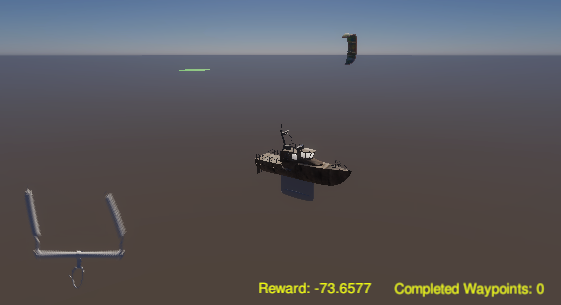
\includegraphics[width=0.8\textwidth]{Images/hard_lock.png}
    \caption{The agent steering on hard lock}
    \label{hard_lock}
\end{figure}


Evaluation of Agent Performance
Explain the methods used to evaluate the trained agent (e.g., test episodes in varied conditions).
Present the results of these evaluations in a systematic manner (e.g., tables, graphs).
Discuss the agent’s ability to generalize from its training to new scenarios.

Comparison with Baselines
If there are baseline models or industry standards, compare your results against these.
Use statistical methods to determine the significance of the results.

Ablation Studies
Discuss any ablation studies conducted (if any) to understand the contribution of different components of the system.
Present the impact of removing/modifying certain parts of the agent or the environment.

Visualizations and Case Studies
Provide visual representations of agent behavior, such as plots of trajectories or state visitation frequencies.
Include screenshots or video stills from Unity to illustrate successful and unsuccessful episodes.

Summary
Sum up the main findings from the results.
Discuss any limitations of these results or the experimental setup.


\section{Evaluation Introduction}
Evaluation
Introduction
Reflect on the purpose of the evaluation.

Methodology for Evaluation
Explain the metrics used to evaluate the agent’s performance.
Describe the process of collecting evaluation data.

Performance Analysis
Analyze the agent’s performance in depth, possibly breaking down by different types of tasks or challenges it faced.
Use statistical methods to discuss the performance variability.

Robustness and Generalization
Evaluate the agent's robustness to changes in the environment (e.g., different wind conditions, system perturbations).
Discuss the agent's ability to generalize from its training environment to similar but unseen environments.

Comparison to Human Performance
If relevant, compare the agent’s performance to that of a human completing the same task.
Discuss any qualitative differences in approaches to the task between the agent and humans.

Discussion of the Evaluation Results
Interpret the results in the context of the project's objectives.
Discuss the strengths and weaknesses of the agent as revealed by the evaluation.

Implications for Future Work
Suggest how the results might inform future projects or the development of RL agents for similar tasks.
Discuss any additional experiments or data that would be valuable.

Conclusion
Summarize the main takeaways from the evaluation.
Discuss the conclusions that can be drawn about the RL agent's performance and the potential for real-world application.